% Sample file on how to use subfiles.
\documentclass[ExampleMasters.tex]{subfiles}

\begin{document}
\clearpage
{\pagestyle{empty}\cleardoublepage}%
\chapter{Verification and validation of steering  (2-3 Seiten)}
\label{chap:testing}

\section{Overview}
In different states of the project different kind of tests were performed. As a first step bench tests were done to verify the developed software. Following that, several tests on the actual dolly, with the dolly in standstill and no trailers connected, were made.

\section{Bench-Testing}
\label{sec:bench-testing}
\subsection{VTM maneuver verification}

For the testing of the vehicle model controllers described in chapter \ref{chap:steering_model} as a first step all the parts were simulated in Simulink. Therefore all parts of the functionality architecture introduced in section \ref{sec:func_architecture} are simulated.
For the \gls{HMI} lookup tables were used for the steering angle and vehicle speed input, so instead of actual driver input a pre-defined maneuver was executed. The \gls{VMM} consists of the vehicle model controller. The steering actuators in the MSD domain were simulated by implementing a first order filter and a time delay, that represents the delay caused by the hydraulic system. For the vehicle plant the \gls{VTM} (see section \ref{sec:VTM}) was used. Figure \ref{fig:funct_architecture_sim} shows how the parts of the functionality architecture are divided to different systems for the simulation of the vehicle model controllers.

\begin{figure*}[!htb]

	\centering
	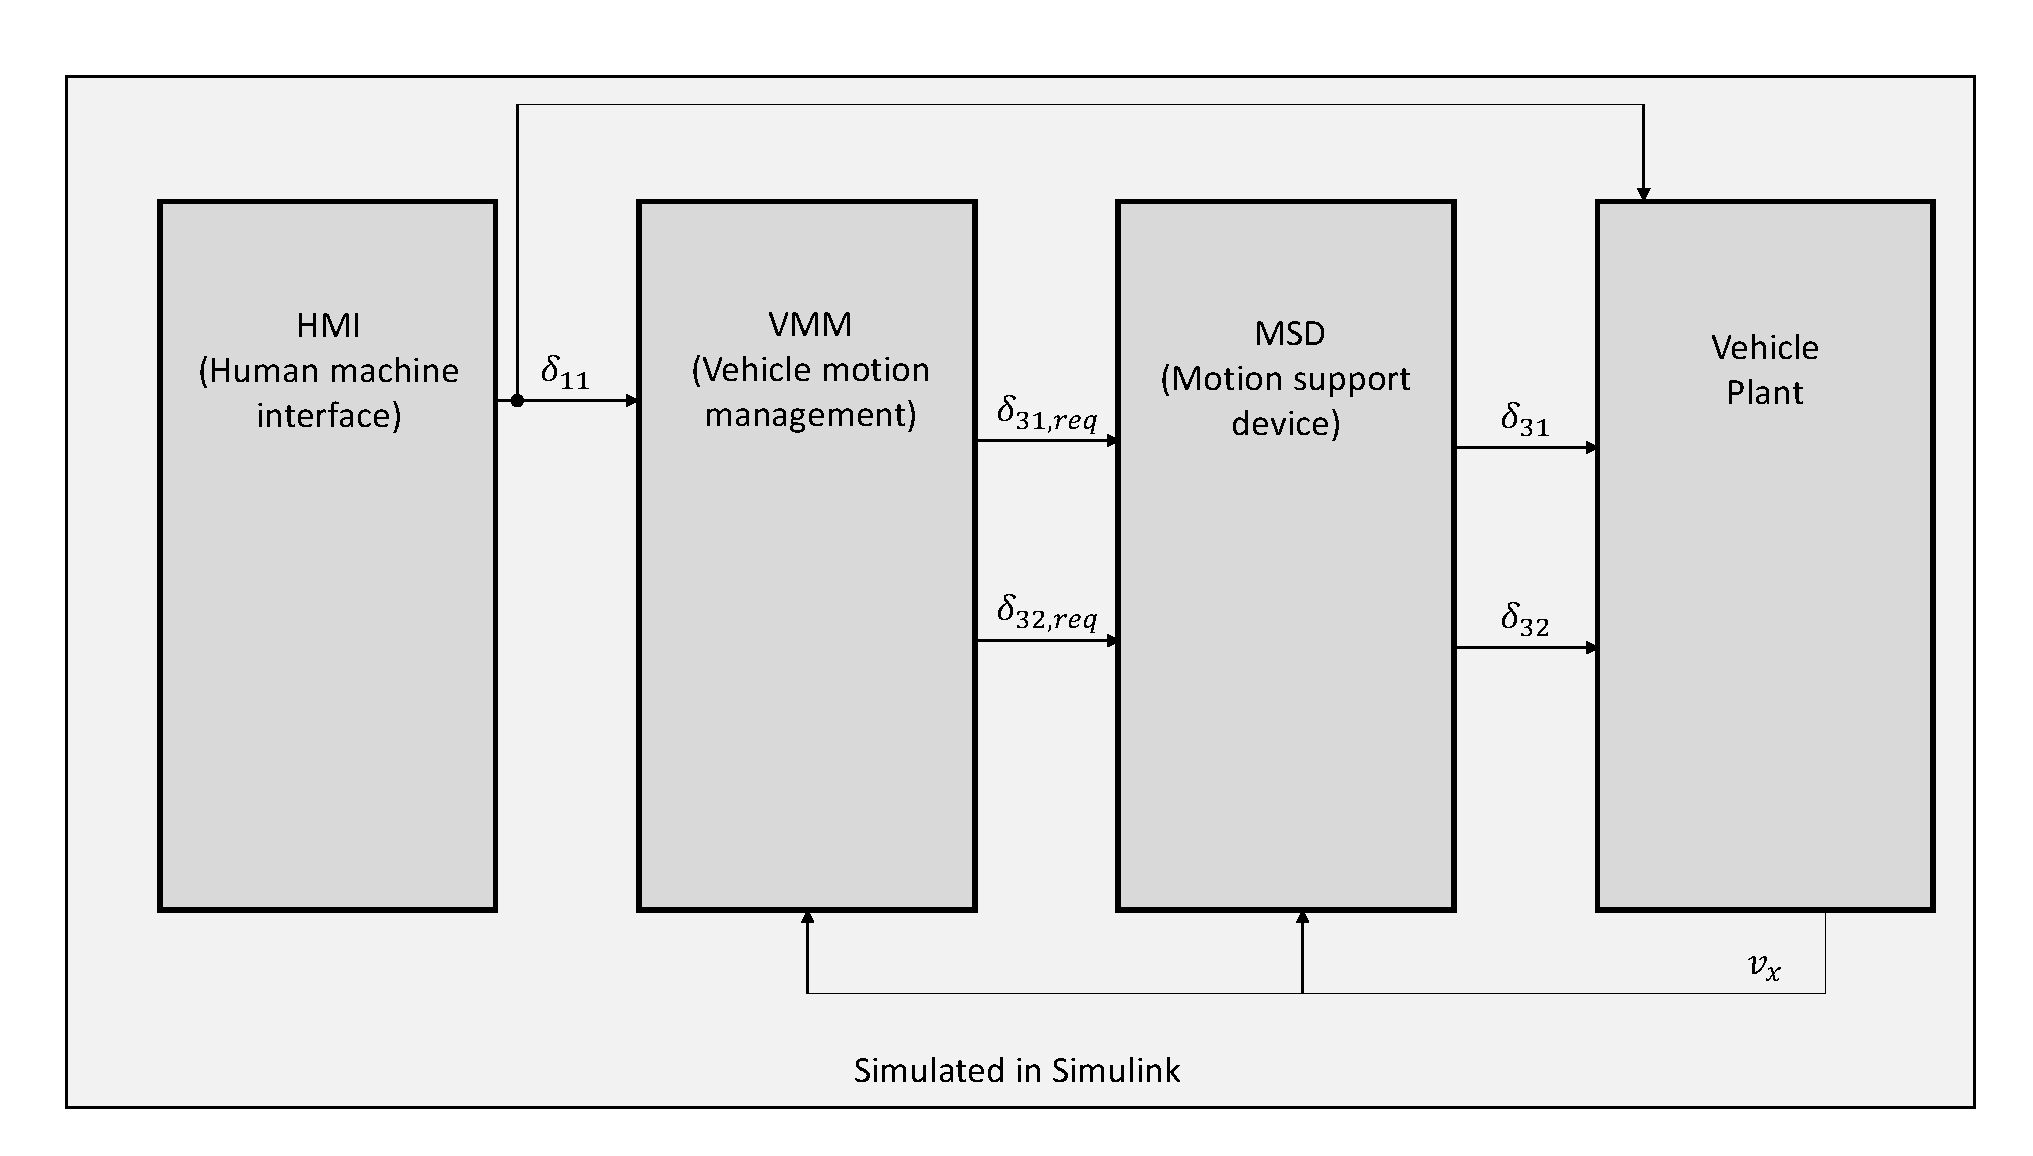
\includegraphics[width=0.5\linewidth]{figures/functionality_architecture_sim}
	
	\caption{Functionality Architecture in simulation}
	\label{fig:funct_architecture_sim}
\end{figure*}\\

\begin{itemize}
	\item include simulation results for maneuver of controller being run inside \gls{VTM} 
	\item perhaps include some picture of the video-output, with the actuated truck
	\item plots for maneuver (steering input, speed over time)
	
\end{itemize}
\subsection{CAN verification}
To test the functionality of the \gls{ASF}-Sensor as a first step it was just connected to power supply and an Arduino with a attached \gls{CAN}-shield. After the \gls{CAN}-message was received successfully with the Arduino, as a next step the sensor's \gls{CAN} pins were connected to the \gls{MABII}. On the \gls{MABII} a simple model, that only contained one \gls{CAN}-Controller with the corresponding dbc-file, was loaded. The bus-monitor tool of ControlDesk, that shows all incoming and outgoing signals on the \gls{CAN} for the corresponding dbc-file, was used to check the sensor signals. 

As outlined in section \ref{sec:interface_with_dolly} the signals generated for each \gls{ETS}-\gls{ECU} need to differ to achieve independent steering. The \gls{CAN}-wiring of the legacy system thus had to be interrupted and split. To ensure that only the correct set of messages was available after the splitting point, Arduino Dues were spliced into the system at all relevant junctions. This was a necessary procedure as gateway-systems between all different \gls{CAN}-subnets on the dolly are in place and needed to be circumvented, which proofed to be a challenging task operating under the maxim of easy revertability to the original state.


\subsection{Fault detection system verification}
\label{sec:fault_detect_test}

\begin{itemize}
	\item send faulty inputs
	\item show plot of faulty input and system reaction
	
\end{itemize}
\section{Processing time evaluation}
\label{chap:processing_time_delay}
\subsection{Background}
The desired solution is supposed to operate at any speed. For high speeds a quick processing and transmission time is required to ensure prompt and realtime intervention of the control system based on the measured input signals. If the delays induced by the different components in the complete system are known or \gls{CAN} be estimated, they can be compensated for in the steering-algorithm running on the rapid-prototyping system.

As outlined in section \ref{sec:measurement_setup} the dolly is equipped with a system to determine the deflection angle of the draw-bar and both the kingpin angles of the \gls{HCT} combination. The sensors' raw signal is then parsed and filtered in an integrated low-level system which feeds the filtered signals to a private \gls{CAN}-bus, where it is picked up by the \gls{MABII}. The filtering operation takes a certain time and thus induces a delay. Furthermore the model running on the rapid-prototyping system needs a certain time to calculate the current desired steering angle for the dollys' wheels. This has to be determined as well. The steering mechanisms on the dolly are also a delay-inducer due to the inertia in the hydro-mechanic system. This is of course unavoidable in any physical system, but when measured can as well to a certain degree be compensated for in the calculations. 

%The measuring chain for the logging solution will also be discussed and the different delays will be discussed. 

\subsection{Measured input delay}
\label{sec:measuring_delay}

The response time of the dolly's steering system was determined in workshop environment in stand-still without any additional axle loads. Tests were conducted for both axles individually to ensure that maximum power was available preventing further delays through insufficient electrical power or hydraulic pressure. A repeated steering angle in the form of a step input was used to determine the reaction time of the system. The step amplitude was increased over different tests to account for possible dependencies on articulation of the steering system. The tests each started and ended with a steering angle of $0^\circ .$ An example for the test sequence can be seen in figure \ref{fig:example_for_step_input_delay_measuring}. Clearly the difference between the requested angle and the actual articulation of the wheel can be seen. Further discussion of the results can be found in section \ref{sec:results_processing_time}.\\

\begin{figure*}
\centering
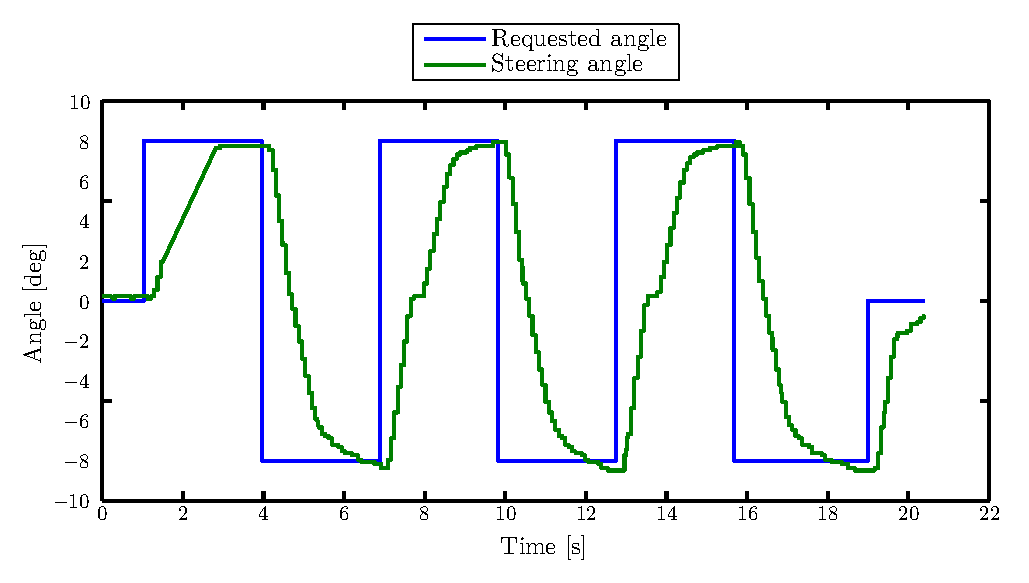
\includegraphics[width=1\linewidth]{figures/example_for_step_input_delay_measuring}
\caption{Example of step input for delay determination, front axle lifted, $8^\circ $ amplitude, six repetitions.}
\label{fig:example_for_step_input_delay_measuring}
\end{figure*}


To eliminate tire friction the investigated axle was suspended in the air in further series of testing by slightly craning up the dolly's front/rear (see figure \ref{fig:dolly_craned_up}) to allow for free movement of the tires. An example for the utilized testing routine can be gathered from table \ref{tab:test_matrx_delay_measuring}. Between the different steps (double amplitude) a sufficient wait time of 3500ms was used to allow the system to reach the requested steering angle. This waiting time was kept constant throughout all tests. \\

	\begin{table}[h]
		
		\centering
		\begin{tabular}{llll}
			\textbf{\#} & \textbf{Amplitude [$  ^\circ $]} & \textbf{Axle}  & \textbf{Comment}                                                                  \\
			1  & 1                & front & lift front axle, \gls{ETS} dead band \\
			2  & 2                & front &                                                                          \\
			3  & 3                & front &                                                                          \\
			4  & 4                & front &                                                                          \\
			5  & 5                & front &                                                                          \\
			6  & 6                & front &                                                                          \\
			7  & 7                & front &                                                                          \\
			8  & 8                & front &                                                                          \\
			9  & 9                & front & error mode, step too\footnotemark[1]                                      \\\hline
			10 & 1                & rear  & lift rear axle, \gls{ETS} dead band  \\
			11 & 2                & rear &                                                                          \\
			12 & 3                & rear &                                                                          \\
			13 & 4                & rear &                                                                          \\
			14 & 5                & rear &                                                                          \\
			15 & 6                & rear &                                                                          \\
			16 & 7                & rear &                                                                          \\
			17 & 8                & rear &                                                                          \\
			18 & 9                & rear & error mode, step too big\footnotemark[1]                                                                   \\
			
		\end{tabular}
		\caption{Test matrix for delay measuring with lifted axle (analogous matrix for non-lifted testing (\#19-\#36))}
		\label{tab:test_matrx_delay_measuring}
	\end{table}
	\footnotetext[1]{If a too big of a step is requested from the steering system, VSE's \gls{ECU} will go into emergency mode. Steering is completely locked, turning the dolly completely passive.}   


As also described in section \ref{sec:results_processing_time} additional response tests were conducted utilizing a ramp input. Here a maximum steering amplitude of $15^\circ $ was used and the slope of the ramp was varied. As the request was not in the form of a step input, no error was triggered like in test \#9 and \#18 (see table \ref{tab:test_matrx_delay_measuring}). The test matrix for this setup is outlined in table \ref{tab:test_matrx_ramp_input}. Besides the changed input-pattern the test- and logging-setup was left unchanged

\begin{table}[h]
	
	\centering
\begin{tabular}{llllll}

 \textbf{\#} &\textbf{ Amplitude [$^\circ$]} & \textbf{Rate} & \textbf{Sample time [s]} & \textbf{Comment} &  \\ 
1	  &  15 & 0.01 & 0.001 &   \\ 
2	  & 15 & 0.001 &  0.001&  \\ 
3	  & 15 & 0.1 &  0.001&   \\ 
4	  & 15 & 0.3 & 	 0.001&   \\ 
5	  & 15 & 0.4 & 0.001 &  error mode, slope too steep\\ 

\end{tabular} 
\caption{Test matrix for delay measurings with ramp input}
\label{tab:test_matrx_ramp_input}	
\end{table}


All testing was automated in ControlDesk using Python scripts to loop through the different tests. The utilized graphical user interface (GUI) \gls{CAN} be seen in figure \ref{fig:control_desk_GUI}. Logging within ControlDesk was started and stopped manually after each test and automatically exported to MATLAB for parsing and analysis. All data was acquired from the steering knuckle sensors originally present in the \gls{ETS}. This sensor's signal is available on the \gls{ETS}-\gls{CAN} (also see section \ref{sec:dolly_system}). 

It was decided to neglect the delays induced by the \gls{CAN} communication. The reason for this is, that both the request as well as the measuring are send over the \gls{CAN}. Which means that the two transmission times are counted with different signs and thus almost exactly cancel out only leaving double the worst case transmission (maximum stuffing bits, worst case arbitration) time as a maximum error of 232$\mu$s. This is sufficiently low regarding the fact, that the simulation on the \gls{MABII} is executed every 0.001s.     



\subsection{Delays in logging measuring chain}
\label{sec:delays_on_arduino}

To have a complete picture of the occuring delays in the measuring chain all relevant bigger execution blocks of the code running cyclically on the Arduino Due to broadcast the \gls{IMU} data to the CAN-bus were evaluated for execution time. Figure \ref{fig:arduino_delays_sketch} gives an overview, into which functions the code was grouped as well as the respectively used protocol for communication. The output via the serial port (\gls{UART}) for visualization purposes on the computer while logging takes very long compared to the execution times of the other depicted code blocks.\footnote{The maximum transmission rate on the \gls{UART} for the Due is 115200bit/s. Transmitting the payload (3x3 sensor axes, signed integer) only excluding all control bits accumulates to 3 sensors x 3 axes x 16bit = 144bit  or 1.25ms}It therefore is disabled while actually logging. 

The delays were evaluated by inserting time-stamped variables into the code before and after each examined function's call. Using the Due's $micros()$ function a resolution in microseonds \gls{CAN} be achieved\footnote{On earlier/smaller Arduinos $micros()$ resolution is 4$\mu$s!} with an accuracy of the inverse of the processors clock frequency (i.e. 11.9ns for the Due). $micros()$' call/execution time was neglected as it is in the magnitude of a couple of dozen nanoseconds. As 

\begin{figure*}[h!]
\centering
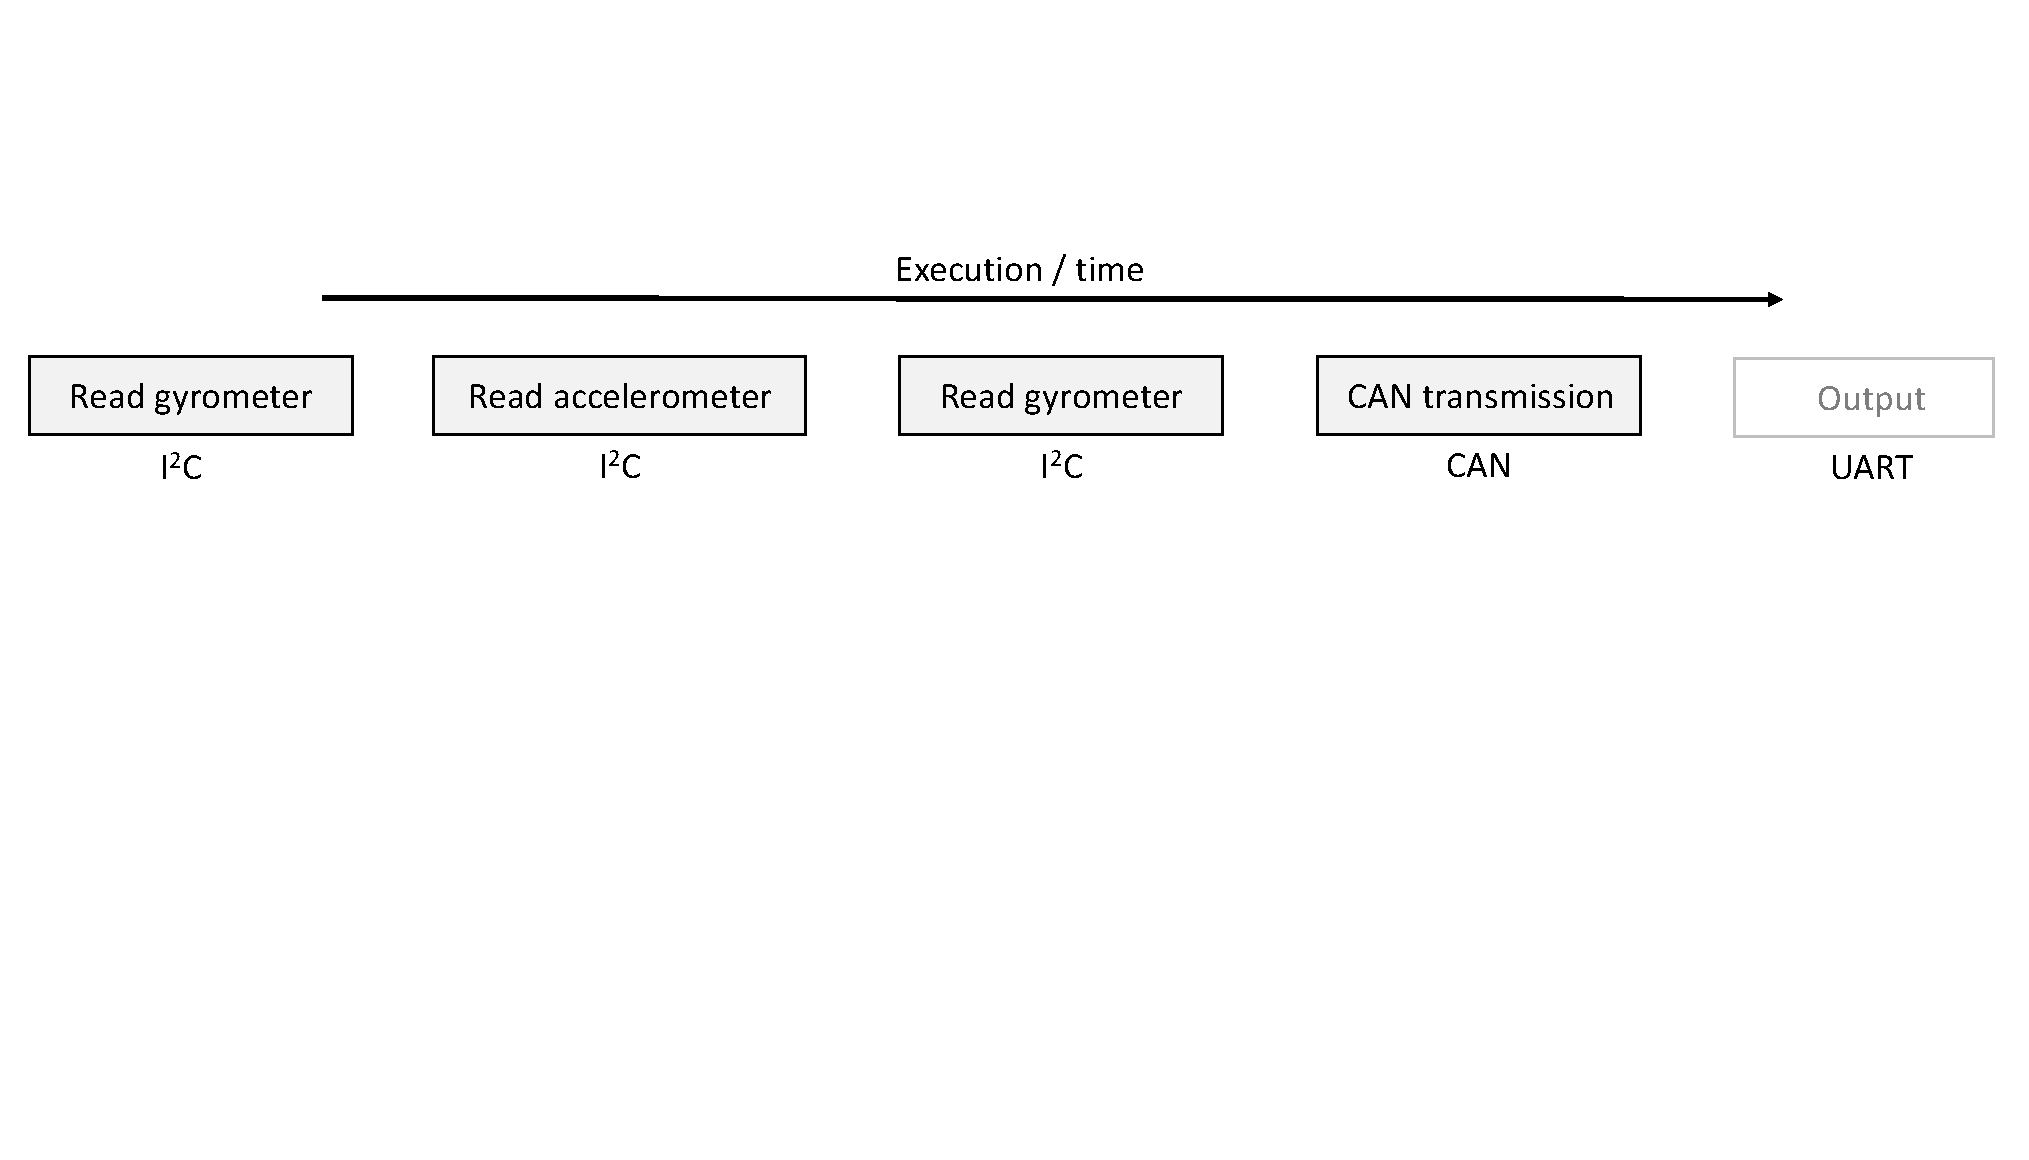
\includegraphics[width=1\linewidth]{figures/arduino_delays_sketch}
\caption{Execution blocks for \gls{IMU} data acquisition on the Arduino Due (overview)}
\label{fig:arduino_delays_sketch}
\end{figure*}


\section{Vehicle testing}
\label{sec:vehicle-testing}

\subsection{System calibration}

The two \gls{ECU}s on the standard \gls{ETS} were calibrated to account for the hardware characteristics before handing-over the legacy system to the active converter dolly project. The parameter set included zeroing of hydraulic pressure levels of the steering system and the integration of the \gls{EBS}-\gls{CAN} signals as well as the articulation angle sensor \gls{CAN} (\gls{ASF}), as it would theoretically be possible to use other sources for the speed-signal needed in the legacy \gls{ETS}. This calibration ensured a correctly and fully working base-system, which in case of failure could be reverted back to. Further on this parameter sets will not be changed to prevent inconsistent behaviour. 

\subsection{Actuator tests}

Actuator tests to verify working hydraulic system for the steering system and correctly pressurized brake-lines as well as normally running \gls{ECU}s receiving correct analog sensor-information (voltage levels) within the legacy \gls{ETS} and \gls{CAN}-signals are possible with \gls{VSE}'s diagnosis screen, that usually sits in the \gls{ETS} locker but was patched out for the \gls{HIL} -tests and during setup in the workshop. As this diagnosis utility ties in directly with the core-functionality it provides a very robust and reliable way to track errors during testing. An example of the home-screen output of the diagnosis display can be seen in figure \ref{fig:ETS_display_homescreen}. Note that it is in "Alarm Mode", which is the fall-back safety level, where all steering cylinders are locked in middle position (i.e. wheels straight). The \gls{ETS} reverts to this state, if sensor information is corrupted or deemed inconsistent. This particular example was triggered by the tests described in section \ref{sec:measuring_delay}.


\begin{figure*}[h]
\centering
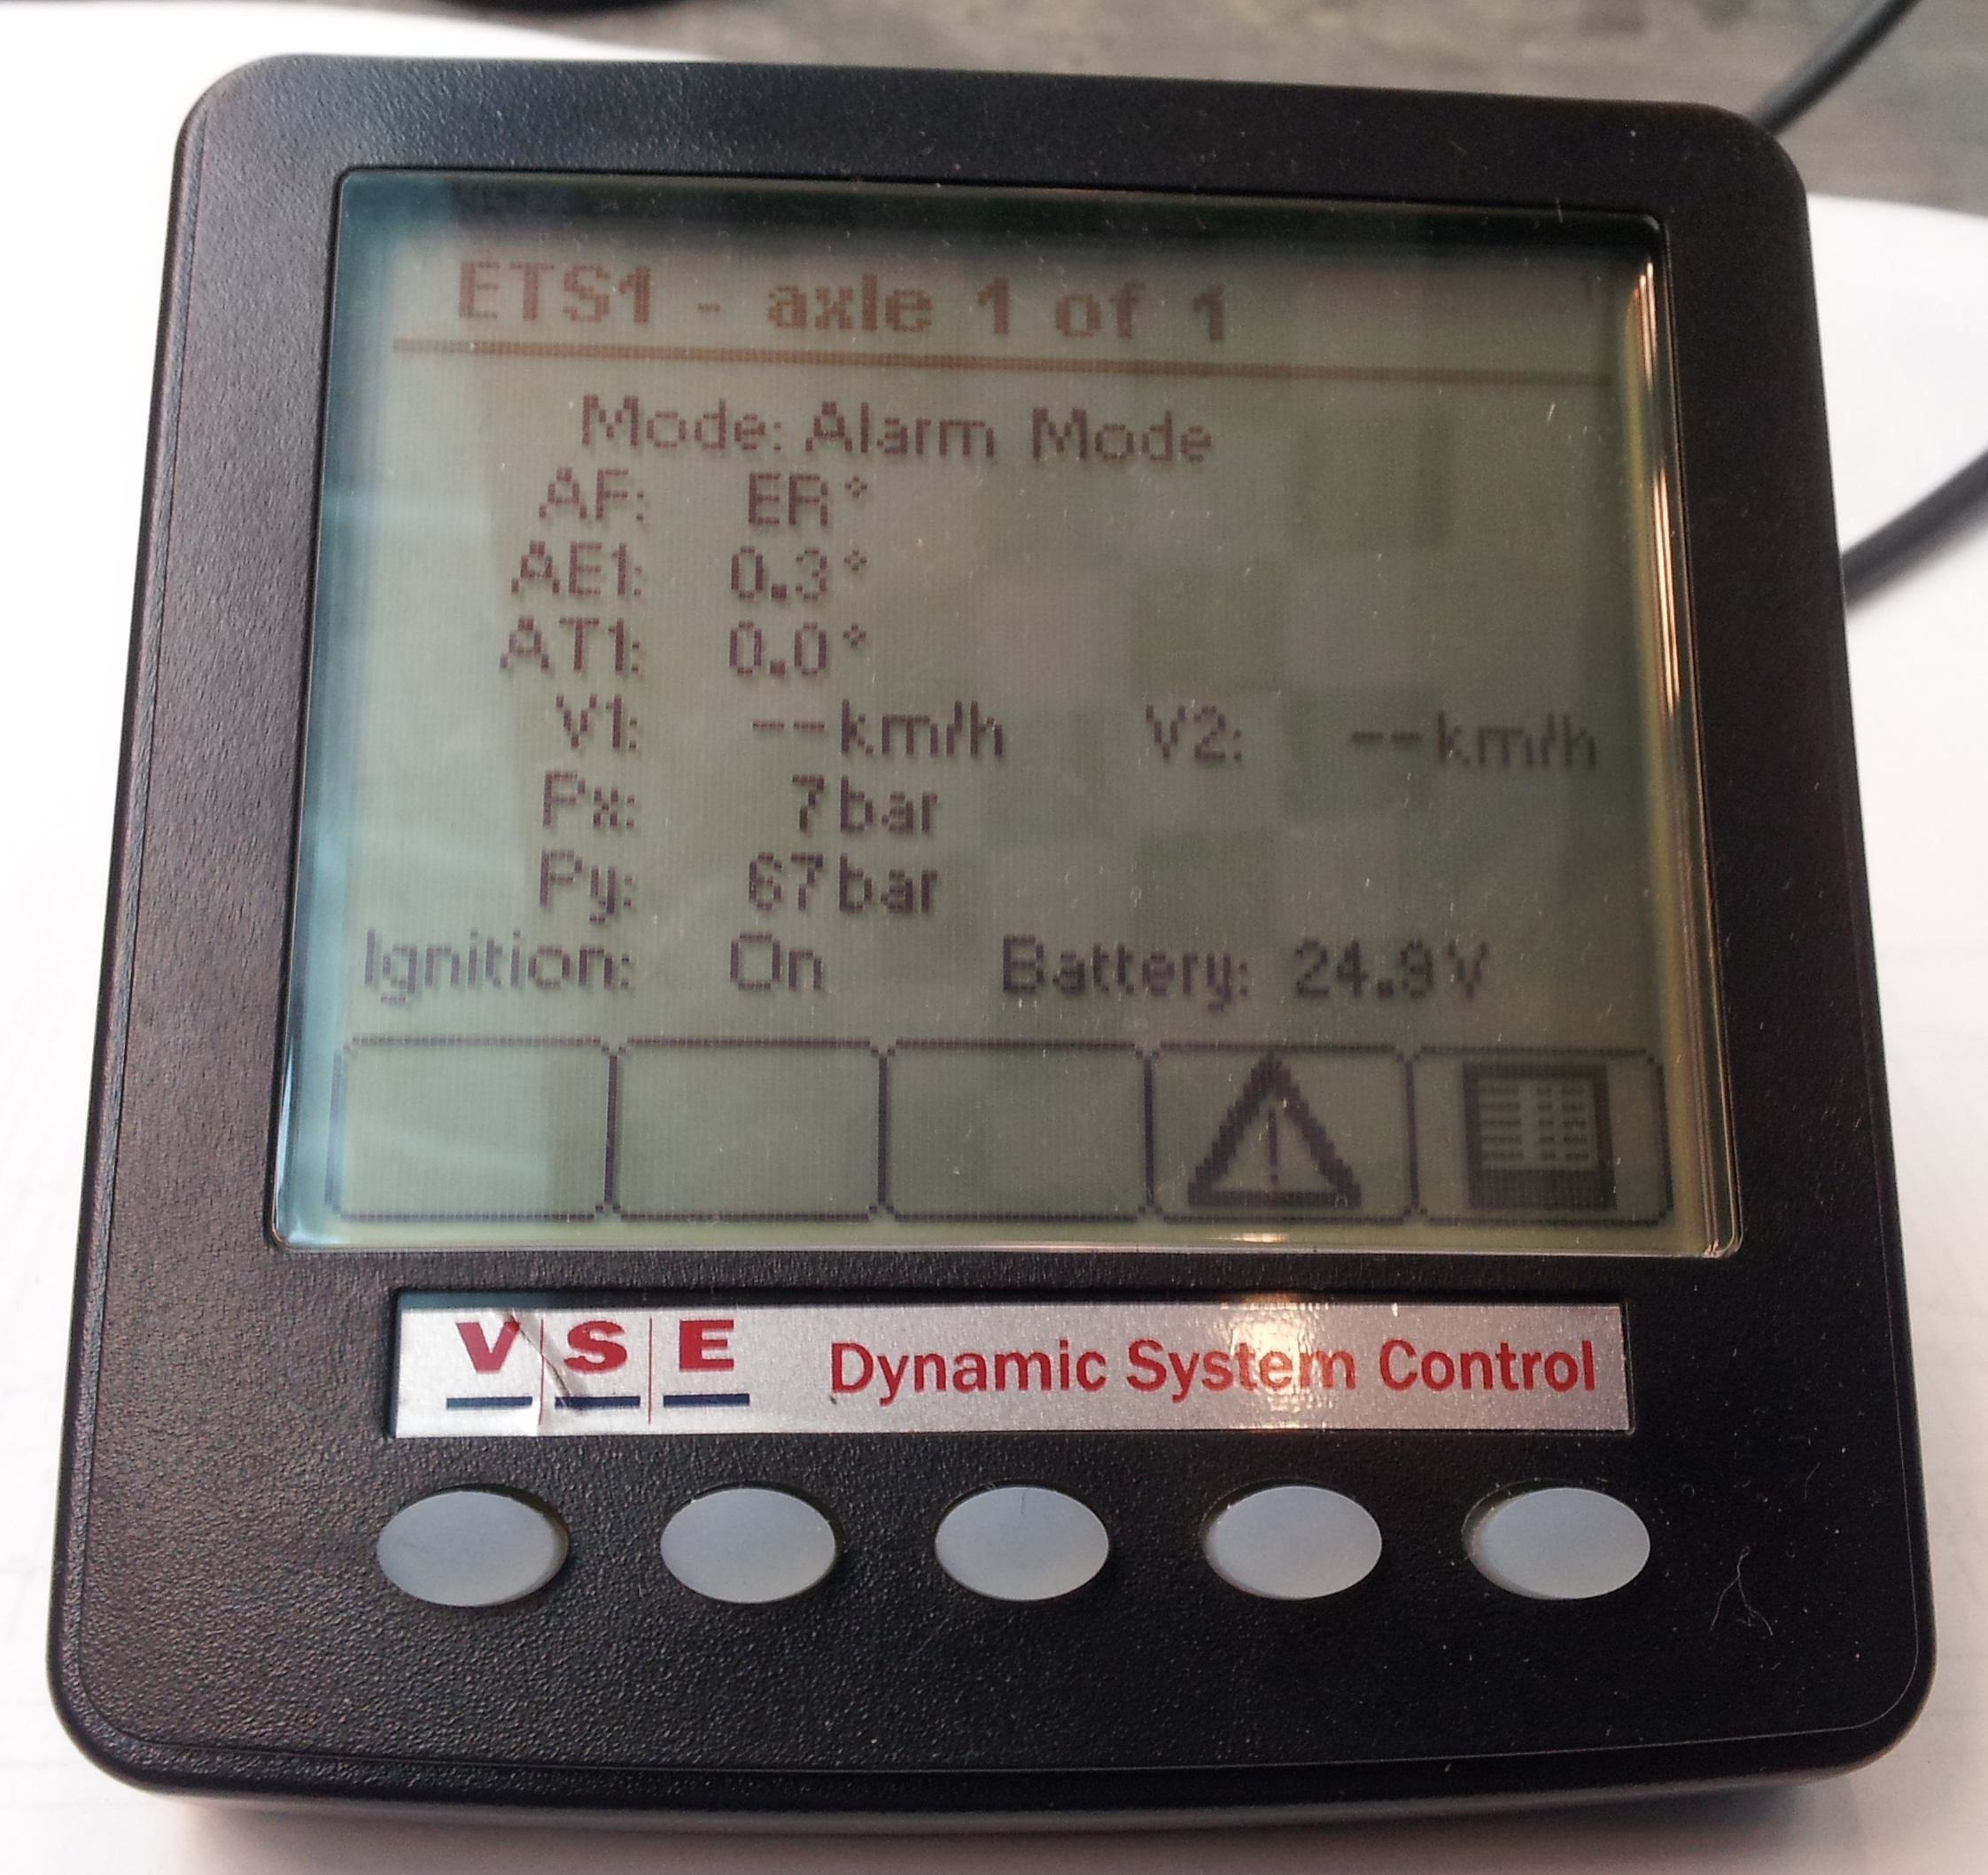
\includegraphics[width=0.6\linewidth]{figures/ETS_display_homescreen}
\caption{\gls{ETS}' diagnosis sceen patched out of the original ETS-locke rto allow easy access during workshop testing. The display is showing the homescreen.}
\label{fig:ETS_display_homescreen}
\end{figure*}

\subsection{Algorithm evaluation}



\subsection{Sensor testing}

The three angle-sensors to determine the articulation between the different independently moving units of the combinations differ in form-factor as they are mounted either on the fifth-wheel turntable or the king-pin respectively, nonetheless all rely on the same measuring principle and broadcast their gathered data in the same fashion on a private \gls{CAN}-bus (refer to figure \ref{fig:dolly_interfaces}). 

As was laid out in section HIER-REF-FUER-BILD-MIT-WEITERFUEHRPARAMETERN! some CAN-messages needed to be patched through to the receiving \gls{ECU} and some had to be changed. It was necessary to run the sensors in bench-tests first to ensure this communication was understood and controllable before implementing it into the final system. The \gls{VSE} sensors need to be connected to 24V \gls{DC} and then independently setup and broadcast the angle of deflection of their turning-plate. The CAN-signal was picked up with a slim Arduino CAN-setup at first to verify the data. In further tests the \gls{CAN}-reception was realized n th \gls{MABII} where subsequently the describes by-pass with modification of selected signals was developed. HIER NOCH EIN BILD VOM SENSOR AM ARDUINO BREADBOARD!!!! Further calibration or testing was not necessary for this sensors, as they are very robust and reliable. 



\begin{itemize}
	\item zero IMUs, make sure paired sensors show the same outputs
	
\end{itemize}

\section{Hardware-in-the-loop testing}
\label{sec:HIL}
\begin{itemize}
	\item description of \gls{HIL} 
	\item Functional architecture diagram (MSD replaced with actual dolly)
	\item Limitations (axle loads, standing still)
\end{itemize}

\gls{VTM} includes a lot of processing heavy sub-models (tire models, vehicle parameter sets) which lead to processing power not sufficing to allow for \gls{VTM} 's execution in the dSpace environment on the \gls{MABII}. To perform \gls{HIL} -testing it was thus necessary to split the comptuational load and accomplish real-time data exchange between the hardware controlling system on the \gls{MABII} and the rest of the simulation which will be run parallely in Simulink in real-time on a standard PC. Though there are dedicated real-time platforms available to achieve real-time execution it was decided to rely on a standard PC to minimize costs and have a lean work-process without extra steps of code conversion to different platforms. Figure \ref{fig:HIL_overview} illustrates the distribution of the \gls{HIL} -setup's different components over two computers, the \gls{MABII} and the actual hardware. 

\begin{figure*}[h]
	\centering
	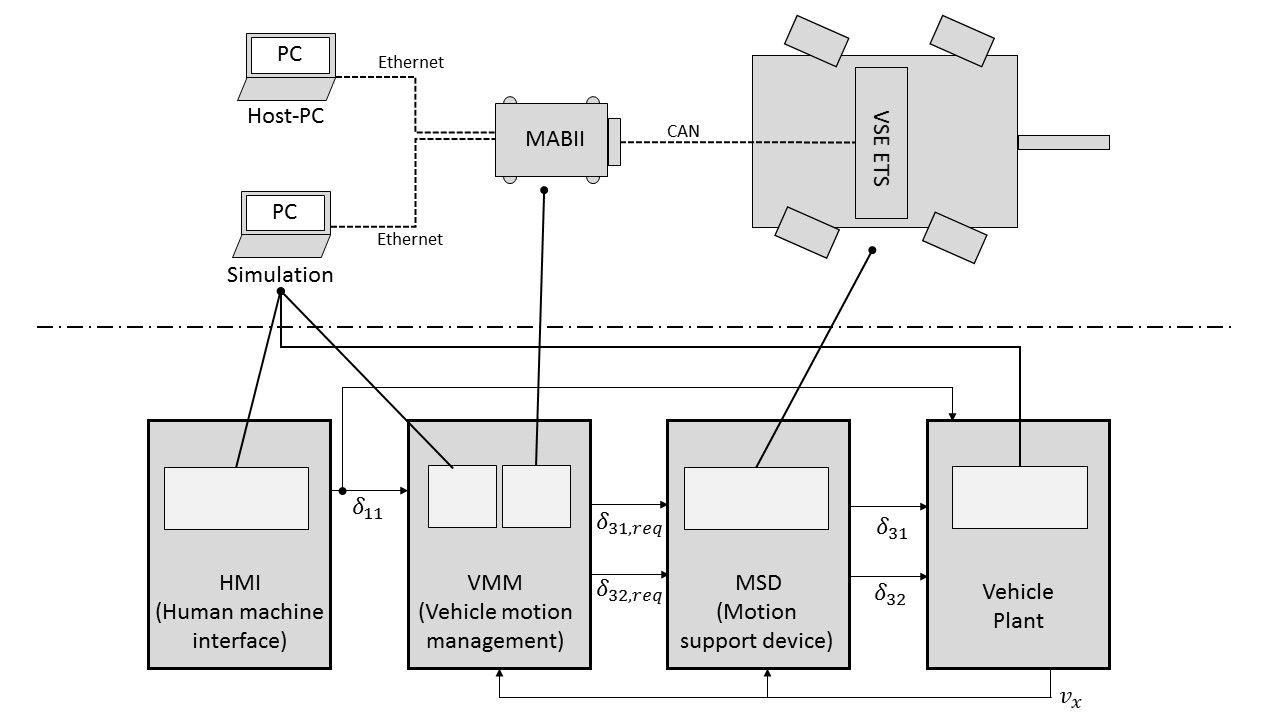
\includegraphics[width=1\linewidth]{figures/HIL_overview}
	\caption{Overview of \gls{HIL} -simulation, distribution of sub-functions over different physical platforms (top) and correlation to Volvo functional architecture (bottom)}
	
	\label{fig:HIL_overview}
\end{figure*}


The Host-PC fulfills the usual task to start-up the dolly and simulation during \gls{HIL}  testing and log the behaviour of the dolly system and the \gls{IMU}s. This is done through the ControlDesk \gls{GUI} which was described in section \ref{sec:control_desk} and of which a screenshot can be found in the appendix (figure \ref{fig:control_desk_GUI}). It already runs the final version of the control and capturing environment and does not require changes for track testing. It is connected to the \gls{MABII} via the Host-PC port.

On the Simulation-PC the simulation of the complete rest of the hardware-system is computed in real-time. Mainly truck, trailers, environment and steering behaviour of the truck are part of this model. All these sub-systems are modeled in \gls{VTM}  which runs on this computer in Simulink. 

Usually Simulink simulations are computed as fast as possible and then afterwards analysis of the results and system's behaviour is conducted offline. This is an unsuitable approach for this thesis' purposes, as it is important to have real-time execution for this sub-system to provide the actual hardware of the \gls{HIL} -test with the needed parameters and simulate the environment at the correct instance also considering the hardware's feedback. I.e. the hardware runs in real-time, so the rest of its environment has to as well. Simulink's Desktop Real-Time toolbox provides the functionality to execute models in real-time on a desktop PC as well as support for a variety of hardware systems. This toolbox was used to connect the MABII's ethernet port to the simulation-PC's ethernet port using the \gls{UDP} protocol. Also part of this toolbox is a sub-packet to access the PC's serial port within the simulation-environment. As it was not possible to receive reliable real-time data via the ethernet-interface which lead to the introduction of the serial interface for the feedback-loop. A similiar setup as decribed in section \ref{sec:arduino} was used to realize the conversion of the CAN-messages directly taken from the \gls{EBS}-\gls{CAN} to serial output on a Arduino Due. As depicted in figure \ref{fig:dolly_split} it is essential to to keep the CAN-buses of the two axles separated to ensure individual steering. Thus two MCP2551 \gls{CAN}-transceivers had to be used for the feedback-loop in the \gls{HIL} -setup.

Limitations: \gls{HIL} -testing took place in workshop environment and thus the dolly was not rolling compromising the tire friction compared with a rolling combination. As outlined in section \ref{sec:results_processing_time} this does not increase the reaction time of the system, though. Furthermore the additional axle load was zero for both axles, as it was not possible to increase the load without a trailer in the lab environment at hand. This is also unlikely to change the results, as is suggested in \ref{sec:results_processing_time} the axle-load is no deciding factor in the wheel articulation's performance. 

The setup for the HIL-testing can also be represented using the functionality architecture introduced in section \ref{sec:func_architecture}.
Compared with the testing of the controllers described in section \ref{sec:bench-testing}, the division of the functionality architecture changed. The MSD are no longer simulated but the actual dolly together with the MABII, which is needed as an interface between the MSD and the other parts of the functionality architecture, is used. The HMI, VMM and vehicle plant are still simulated in Simulink. Figure \ref{fig:funct_architecture_hil} shows how the parts are divided to different systems.
\begin{figure*}[!htb]
	\centering
	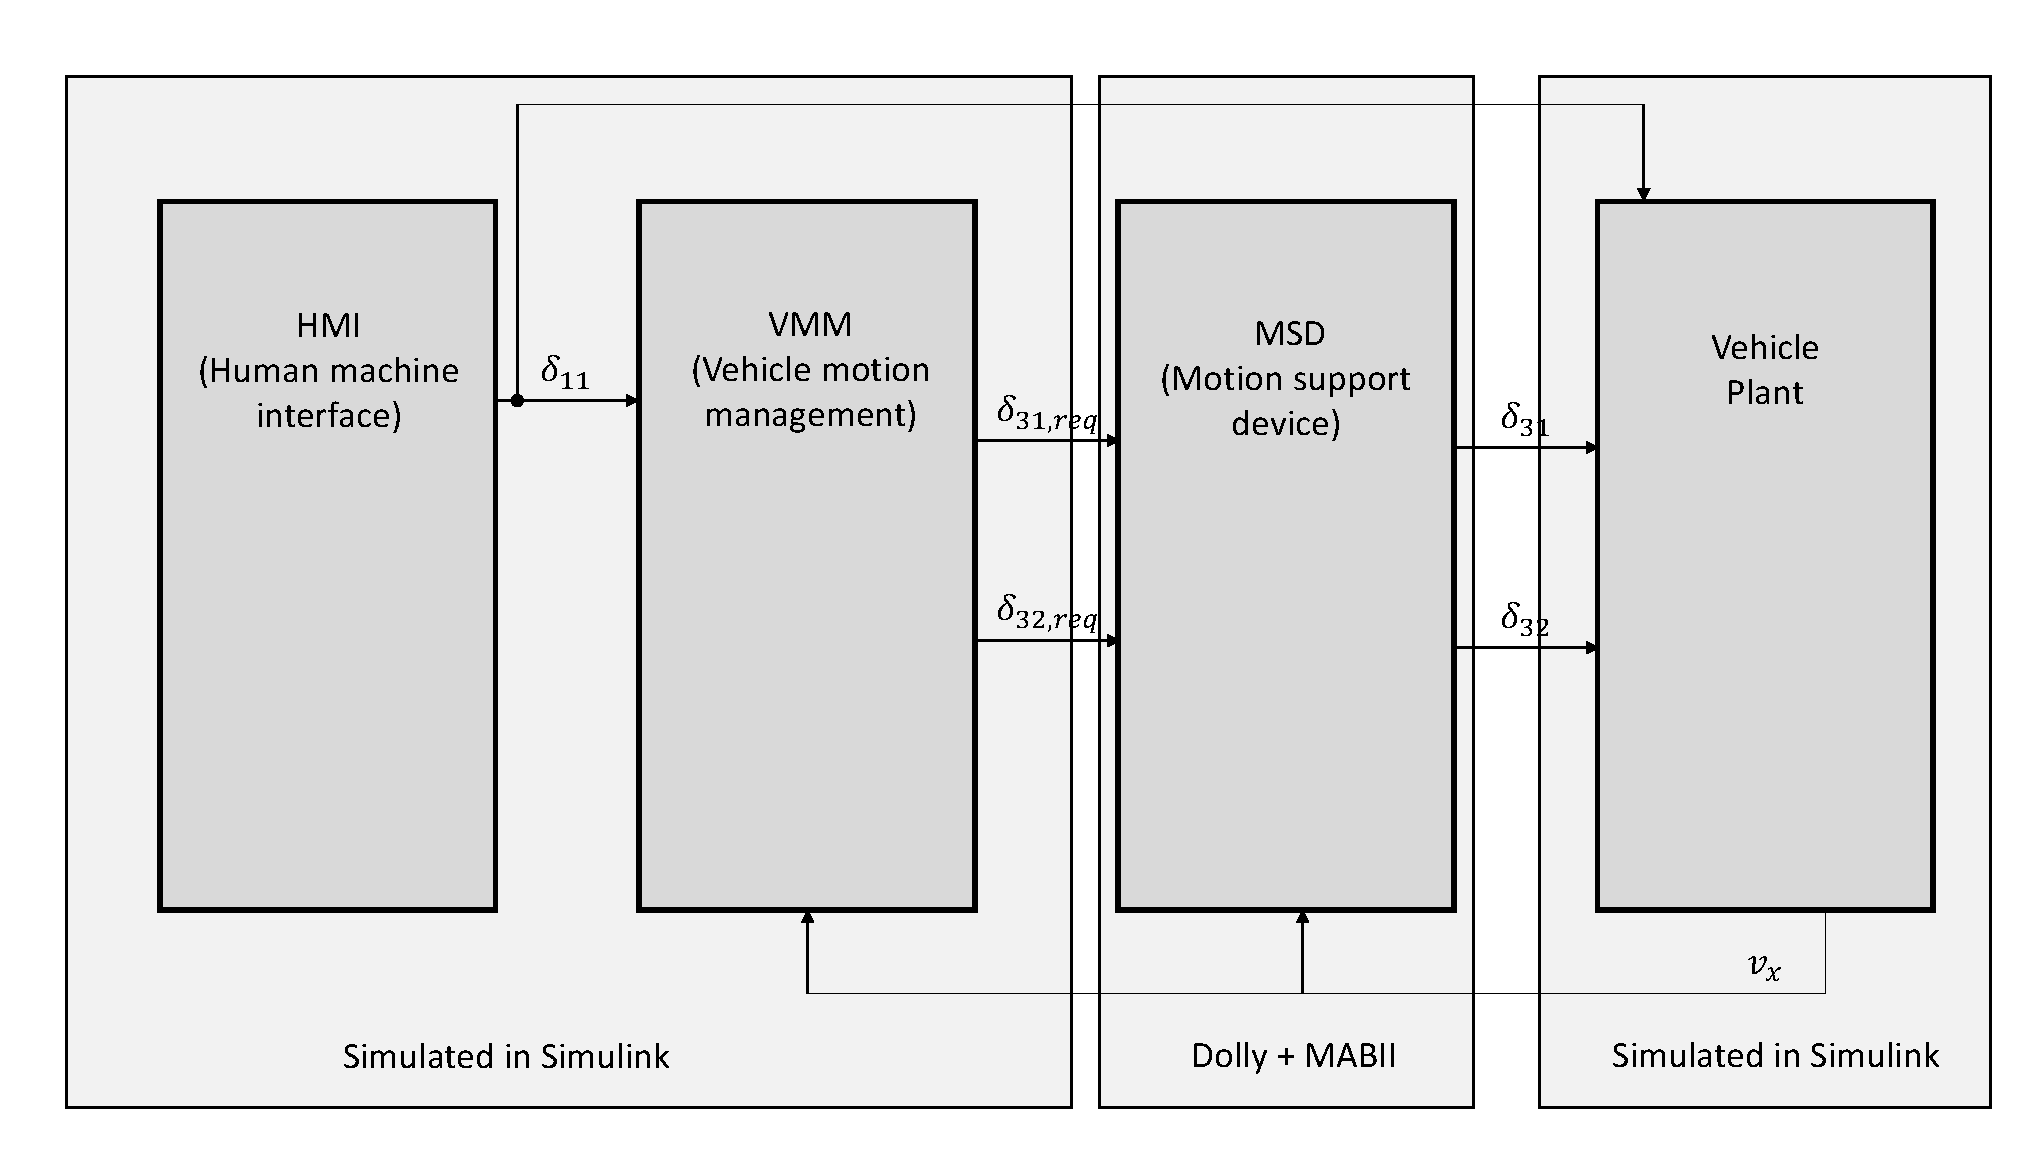
\includegraphics[width=0.5\linewidth]{figures/functionality_architecture_hil}
	
	\caption{Functionality Architecture for HIL-testing}
	\label{fig:funct_architecture_hil}
\end{figure*}\\

\subsection{Low-speed controller}
The maneuver that was used for testing the Low-speed controller was a 180 degree turn at constant speed. The steering angle of the tractor can be seen in Figure \ref{fig:HIL002_delta11}.\\
\begin{figure*}[!htb]
	\centering
	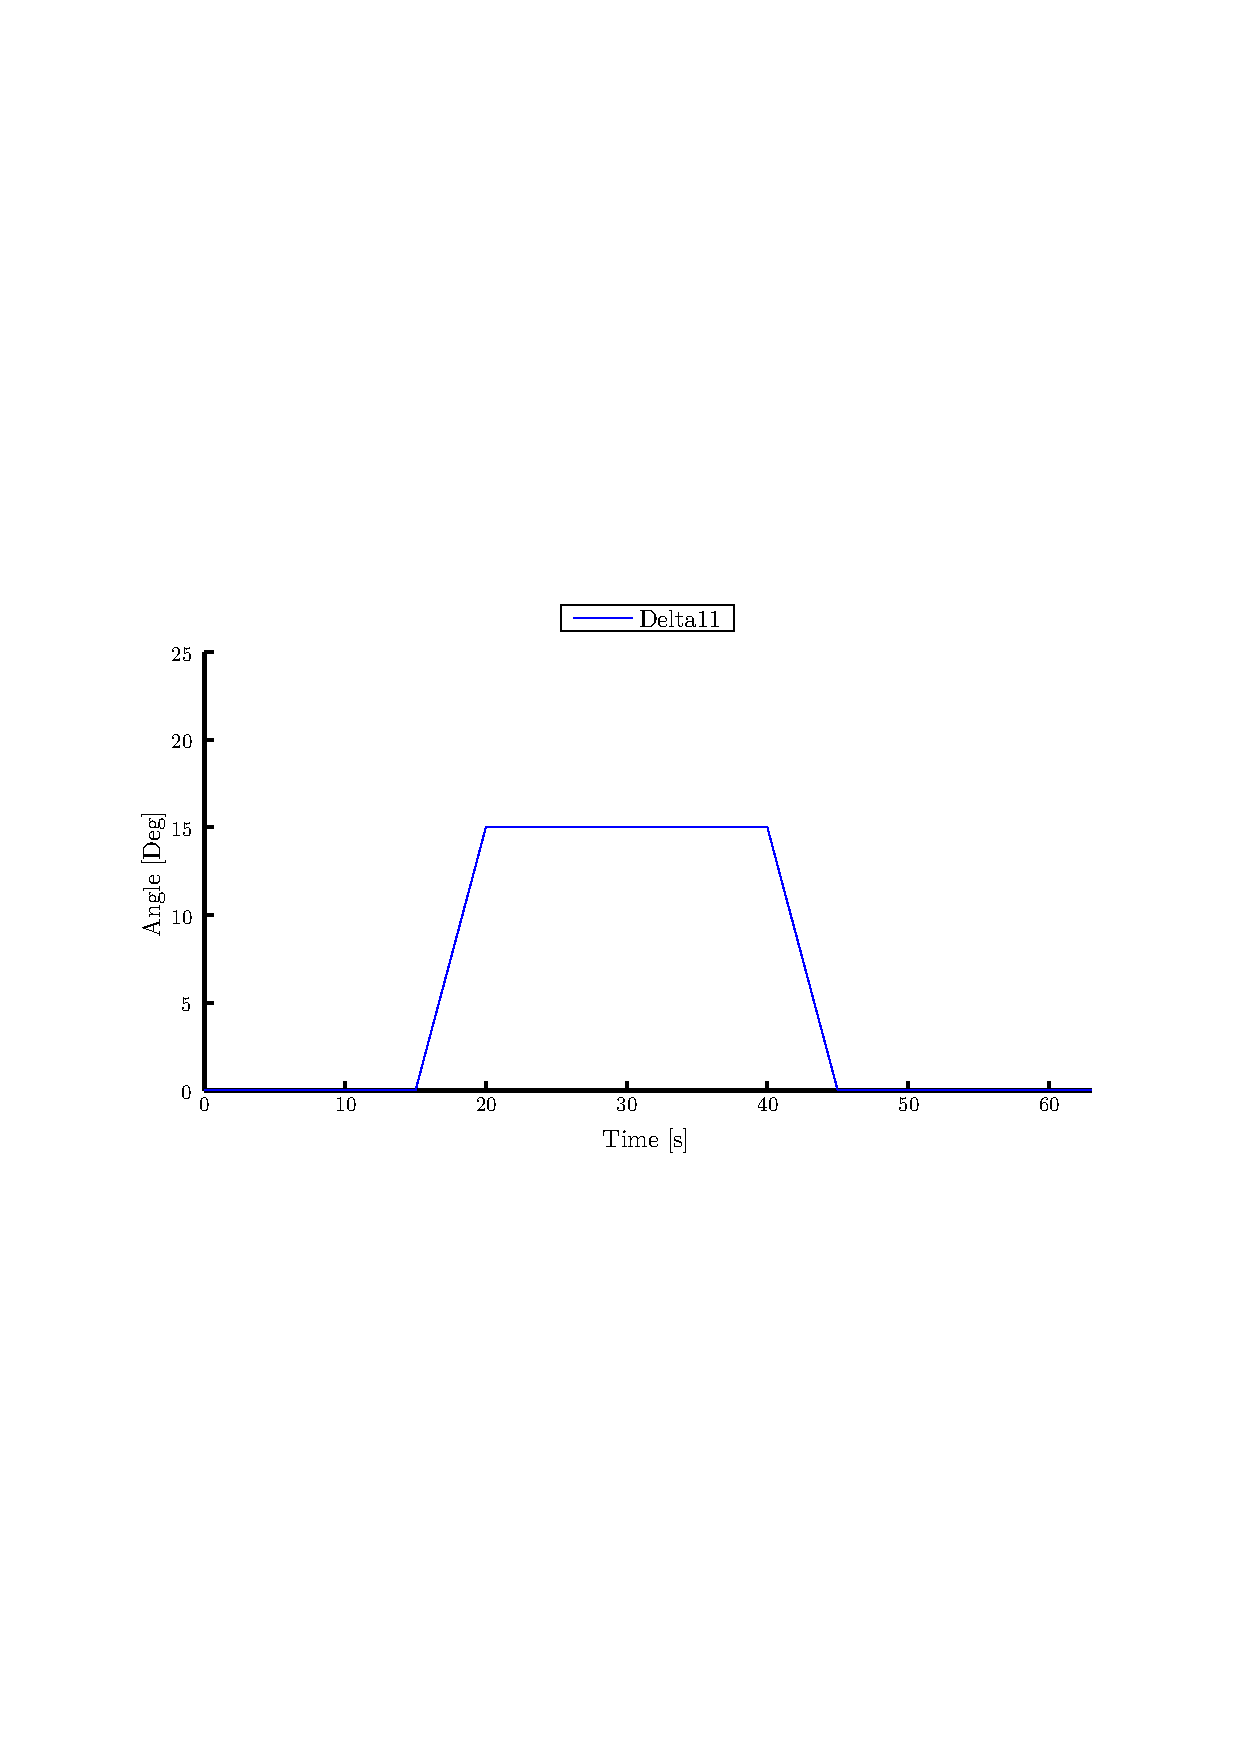
\includegraphics[width=1\linewidth]{figures/HIL_delta11}
	\caption{HIL test steering angle tractor}
	
	\label{fig:HIL002_delta11}
\end{figure*}
As a first step a very simple controller was used for controlling the steering of the dolly. The controller used the articulation angle between the first semitrailer and the dolly as an input. The output to both axles was this angle multiplied with a gain of 4.



\subsection{High-speed controller}

\section{Track testing}
\label{sec:track-testing}
For testing on a test track the different parts of the  functionality architecture (see section \ref{sec:func_architecture}) will be handled as follows:
Since a complete vehicle combination will be used for track testing, this corresponds to the vehicle plant of the functionality architecture. The HMI domain is represented by the driver of the vehicle. The VMM is running on the MABII, which works as an interface between the VMM, the dolly and the vehicle. Figure \ref{fig:funct_architecture_track} shows how the parts are divided to different systems.
\begin{figure*}[!htb]
	\centering
	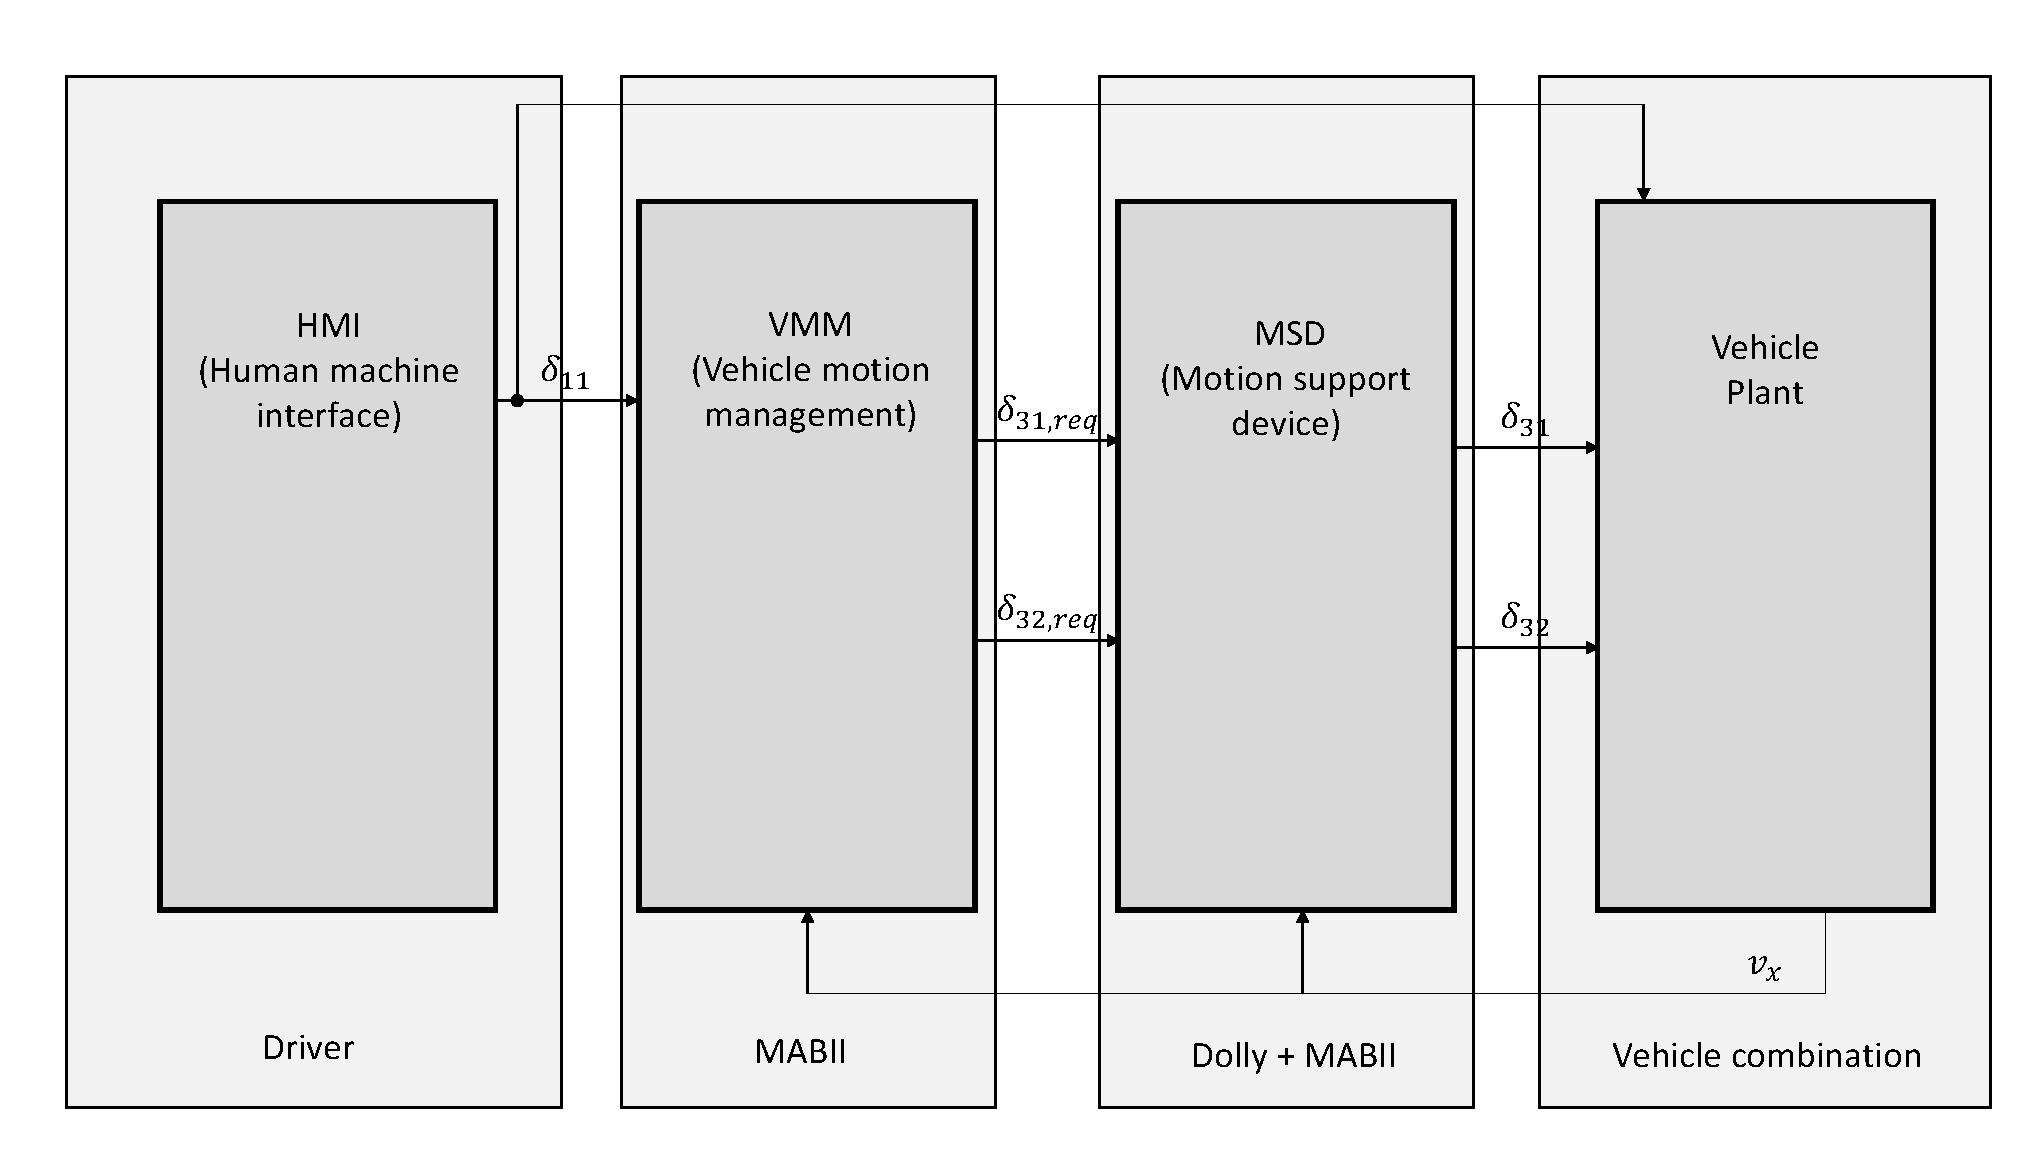
\includegraphics[width=0.5\linewidth]{figures/functionality_architecture_track}
	
	\caption{Functionality Architecture on track testing}
	\label{fig:funct_architecture_track}
\end{figure*} 
\subsection{Testmaneuvers}

\begin{itemize}
	\item lit research for standard maneuvers
	\item sine-wave
	\item outline critical parts of maneuver
	\item figure with SA over time
	\item expected behaviour from simulation
\end{itemize}

\subsection{Testenvironment AstaZero}

\begin{itemize}
	\item overview of AZ
	\item map in appendix?
	\item restrictions of environment
	
\end{itemize}

\subsection{Testmatrix}

\begin{itemize}
	\item checklist for launch
	\item parameters that very varied
	\item different runs
	\item planned maneuvers
	
\end{itemize}

\subsection{Test setup and instrumentation}

\begin{itemize}
	\item detailed description of placement of sensors, wiring, logging-PC
\end{itemize}


\end{document}
